\section*{\hfil Project Description \hfil}
\vspace{-16pt}
\noindent\hrulefill
% From solicitation NSF 22-586: 
% https://nsf-gov-resources.nsf.gov/solicitations/pubs/2022/nsf22586/nsf22586.pdf?VersionId=zhHYrr4DGF8u3J8kV3r217ygkg4.fKRM 
%The Project Description section should contain a well-argued and specific proposal for activities that will, over a 5-year period, build a rm foundation for a lifetime of contributions to research and education in the context of the Principal Investigator's organization. The proposed project should aim to advance the employee's career goals and job responsibilities as well as the mission of the department or organization. The Project Description may not exceed 15 pages.
%The Project Description should include: 
% a description of the proposed research project, including preliminary supporting data where appropriate, specific objectives, methods and procedures to be used, and expected significance of the results; 
% a description of the proposed educational activities and their intended impact; 
% a description of how the research and educational activities are integrated or synergistic; 
% a description of other broader impacts, besides the education activities, that will accrue from the project; 
% and results of prior NSF support, if applicable.
%Successful applicants will propose creative, effective research and education plans, along with strategies for assessing these components. The proposed activities should help applicants develop in their careers as both outstanding researchers and educators. While excellence in both education and research is expected, activity of an intensity that leads to an unreasonable workload is not. The research and educational activities do not need to be addressed separately if the relationship between the two is such that the presentation of the integrated project is better served by interspersing the two throughout the Project Description.
%
%
%
%%
% Objectives, Goals, and Tasks
%%
%
% Goals and Objectives are not interchangeable. Think about your research goal, then state your research objectives and the tasks that need to be done to achieve the objectives.
%		Goal – A statement of what you are trying to achieve.
%		Objective(s) – Clearly defined step(s) towards your goal.
%		Tasks – Activities to achieve objective(s)


\vspace{-10pt}
\section{Motivation \& Objectives}

\lipsum[3]

%%%%%%%%%%%%%%%
% RESEARCH OBJECTIVES 
%%%%%%%%%%%%%%%
\begin{enumerate}[label=\textbf{RO~\arabic*.},leftmargin=2cm]

\vspace{-8pt}
\item Achieve bigness

\vspace{-10pt}
\item Achieve fireball power

\vspace{-10pt}
\item Save the prisoner

\end{enumerate}

\lipsum[1]

\setlength{\intextsep}{5pt}  % reduce top/bottom margin from this wrapfig
\begin{wrapfigure}{R}{0.5\textwidth}
	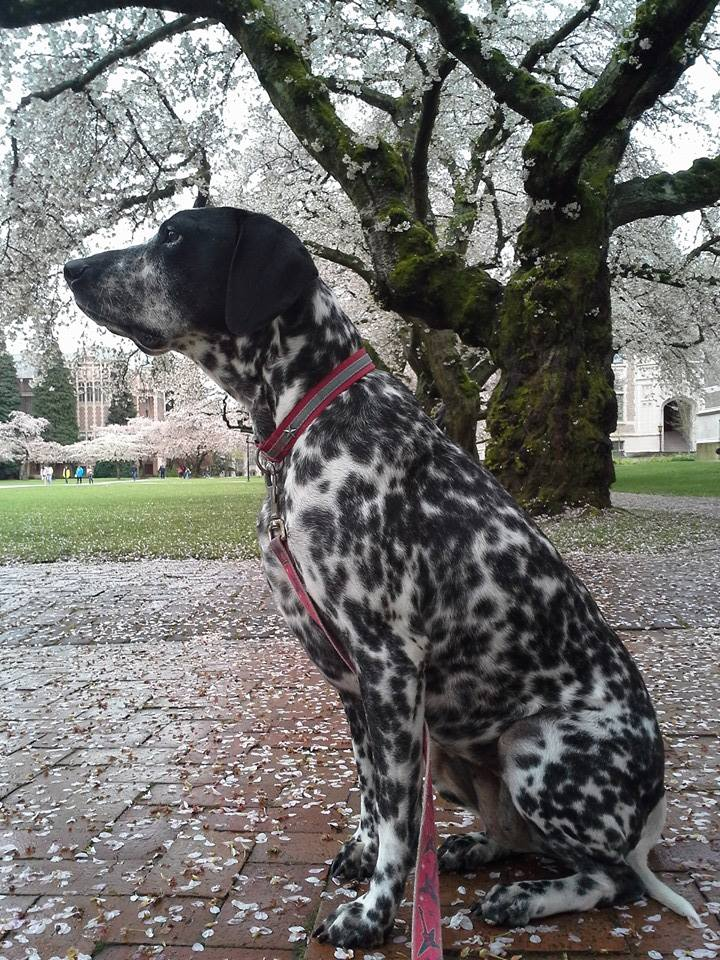
\includegraphics[width=0.5\textwidth]{maggieinthethespring.jpg}
	\caption{\textit{A dog under a blossoming cherry tree.}}
\end{wrapfigure}






\section{Background and motivation}

\lipsum




\section{Proposed Study \& Research Plan}

\lipsum[1]



% Set the subsection to be preceded by RO
\renewcommand{\thesubsection}{\arabic{section}.RO-\arabic{subsection}}

\subsection{Achieve bigness}
\label{sec:RO1}
\vspace{-6pt}

\textit{We will find a mushroom and eat it to grow big.}



\vspace{-10pt}
\subsubsection{Rationale and significance of RO-1}
\vspace{-6pt}

\lipsum[2]




\vspace{-10pt}
\subsubsection{Implementation plan for RO-1}
\vspace{-6pt}


\paragraph*{Task RO-1.A: Run to the right}
\lipsum[1]

\paragraph*{Task RO-1.B: Jump up and hit block}
\lipsum[1]

\paragraph*{Task RO-1.C: Co-occupy the space of the mushroom}
\lipsum[1]

\vspace{-10pt}
\subsubsection{Evaluation plan for RO-1}

\vspace{-8pt}
\paragraph*{Formative evaluation:} 
\lipsum[1]

\vspace{-14pt}
\paragraph*{Summative evaluation:} 
\lipsum[1]


\vspace{-10pt}
\subsubsection{Summary of expected results of RO-1}
\vspace{-6pt}

\lipsum[1]












%Research Objective 2
%•	Task 1 (or R1)
%•	Task 2 (or R2)
%•	…

\bigskip
\vspace{-10pt}
\subsection{Achieve fireball power}
\label{sec:RO2}
\vspace{-6pt}

\textit{We will find a glowing flower and meld with it to get fireball power.}




\vspace{-10pt}
\subsubsection{Rationale and significance of RO-2}
\vspace{-6pt}

\lipsum[2]

\vspace{-10pt}
\subsubsection{Implementation plan for RO-2} 
\label{sec:RO2plan}

\vspace{-6pt}
\paragraph*{Task RO-2.A: Jump onto a turtle}
\lipsum[1]

\vspace{-6pt}
\paragraph*{Task RO-2.B: Kick the turtle into a block}
\lipsum[1]

\vspace{-6pt}
\paragraph*{Task RO-2.C: Occupy the same space as the flower}
\lipsum[1]

\vspace{-10pt}
\subsubsection{Evaluation plan for RO-2}

\vspace{-8pt}
\paragraph*{Formative evaluation:}  
\lipsum[1]


\vspace{-14pt}
\paragraph*{Summative evaluation:}  
\lipsum[1]



\vspace{-10pt}
\subsubsection{Summary of expected results of RO-2}
\vspace{-6pt}

\lipsum[1]





%Research Objective 3
%•	Task 1 (or R1)
%•	Task 2 (or R2)
%•	…

\bigskip
\vspace{-10pt}
\subsection{Save the prisoner}
\label{sec:RO3}
\vspace{-6pt}

\textit{We will find the captured innocent person and save them.}


\vspace{-10pt}
\subsubsection{Rationale and significance of RO-3}
\vspace{-6pt}
\lipsum[2]

\vspace{-10pt}
\subsubsection{Implementation plan for RO-3} 

\vspace{-6pt}
\paragraph*{Task RO-3.A: Enter the castle}
\lipsum[1]

\vspace{-6pt}
\paragraph*{Task RO-3.B: Navigate to the Boss}
\lipsum[1]

\vspace{-6pt}
\paragraph*{Task RO-3.C: Defeat the Boss}
\lipsum[1]

\vspace{-10pt}
\subsubsection{Evaluation plan for RO-3}

\vspace{-8pt}
\paragraph*{Formative evaluation:}  
\lipsum[1]

\vspace{-14pt}
\paragraph*{Summative evaluation:} 
\lipsum[1]


\vspace{-10pt}
\subsubsection{Summary of expected results from RO-3}
\vspace{-6pt}

\lipsum[1]


% Reset subsection numbering back to normal
\renewcommand{\thesubsection}{\arabic{section}.\arabic{subsection}}


\newpage
\section{Broader Impacts of the Proposed Work}
\label{sec:BI}

\lipsum


\section{Timeline}


\begin{figure}[H]
	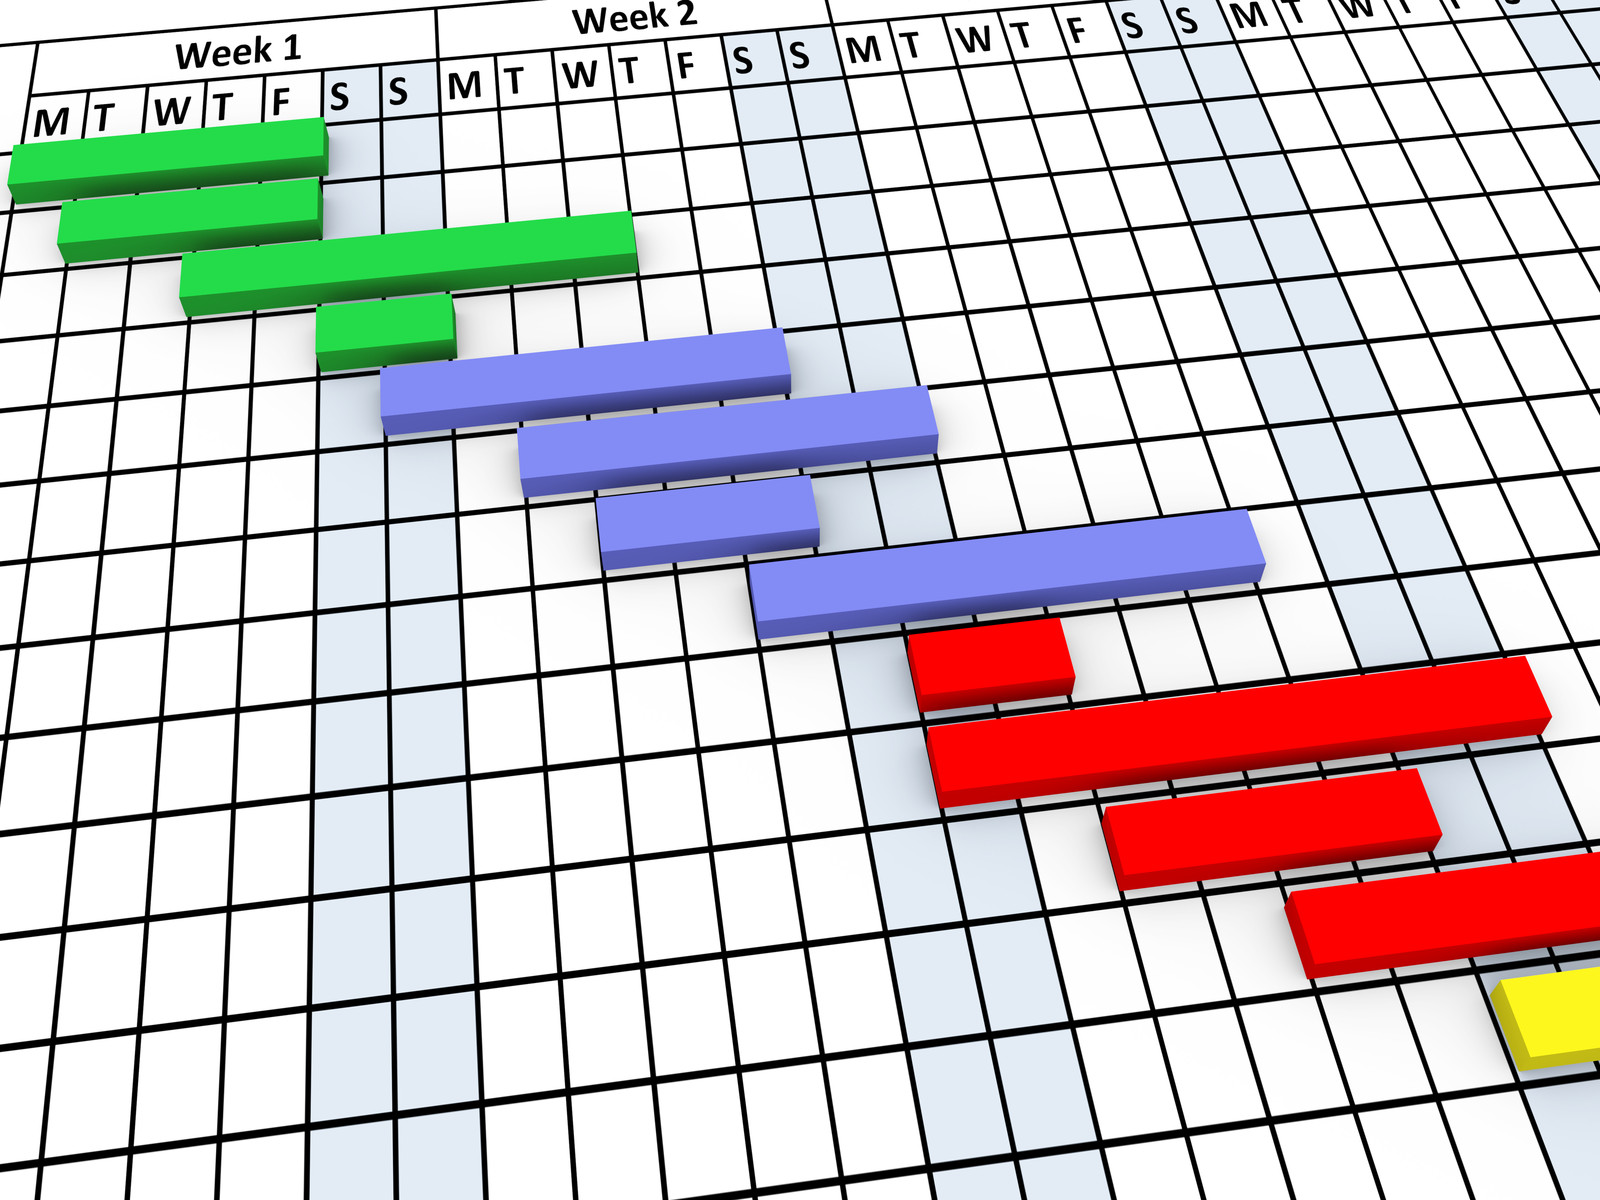
\includegraphics[width=\textwidth]{gantt.jpg}
	\label{fig:gantt}
	\vspace{-10pt}
	\caption{\textit{Timeline for planned completion of the proposed work.}}
\end{figure}

\lipsum[2]


\section{Results from Prior NSF Support}
%If any PI or co-PI identified on the project has received NSF funding (including any current funding) in the past five years, in formation on the award(s) is required, irrespective of whether the support was directly related to the proposal or not.
%In cases where the PI or co-PI has received more than one award (excluding amendments), they need only report on the one award most closely related to the proposal. Funding includes not just salary support, but any funding awarded by NSF. The following information must be provided:\\

\noindent \emph{\underline{Name of PI}}: NSF-Program (Award Number) ``Title of the Project'' (\$AMOUNT, PERIOD OF SUPPORT). 
{\bf Publications:} List of publications resulting from the NSF award. A complete bibliographic citation for each publication must be provided either in this section or in the References Cited section of the proposal); if none, state: ``No publications were produced under this award.'' {\bf Research Products:} evidence of research products and their availability, including, but not limited to: data, publications, samples, physical collections, software, and models, as described in any Data Management Plan.

% evidence of research products and their availability, including, but not limited to: data, publications, samples, physical collections, software, and models, as described in any Data Management Plan.

